\documentclass{article}
\usepackage{amsmath, amssymb, tikz, geometry, graphicx, natbib, mwe, xcolor,
 listings, tabularx, pdfpages, blindtext, mathtools, stackengine, amsthm, pgfplots,bigints, relsize, upgreek, esint, array}
\usepackage{hyperref}
\usepackage{slashed, enumitem}

\pgfplotsset{width=10cm,compat=1.9}

\colorlet{myWhite}{white!35!gray}
\definecolor{background}{HTML}{181818}

\hypersetup{
    colorlinks=true,
    linkcolor=violet,
    filecolor=magenta,      
    urlcolor=cyan,
    pdftitle={Overleaf Example},
    pdfpagemode=FullScreen,
}

\geometry{ 
 a4paper,
 total={170mm,257mm},
 left=20mm,
 top=10mm,
 }
 
\lstdefinestyle{mystyle}{ 
bracketsstyle=\color{red}
}

\title{Elettrotecnica}
\author{Giuseppe Bumma}


%----------------------------------------------------------------------
%use this for a total black background
%\pagecolor{black}
%\color{myWhite}
%----------------------------------------------------------------------



% use this for a shade of gray background
\pagecolor{background}
\color{myWhite}



\begin{document}

%Commands
\newcommand{\R}{\mathbb{R}}
\newcommand{\bb}[1]{\mathbb{#1}}
\newcommand{\cc}[1]{\mathcal{#1}}
\newcommand{ \lognormal }{\text{Lognormal} }
\newcommand{\tb}[1]{\textbf{#1}}
\newcommand*\circled[1]{\tikz[baseline=(char.base)]{%
            \node[shape=circle,draw,inner sep=2pt] (char) {#1};}}
%for using circled number in enumerate use:
%\begin{enumerate}[label=\protect\circled{\arabic*}]


\tableofcontents

\maketitle

\section{Introduzione}

\subsection{La carica elettrica e la forza di Coulomb}
Se due particelle cariche, supposte puntiformi, di carica $q_0$ e $q_1$, siano a una distanza finita fra loro nel vuoto, la \textbf{legge di Coulomb} descrive la forza elettrostatica interagente fra loro:
\[
    |F_C| \propto \frac{q_1q_2}{e^2}
\]
con $r$ distanza tra le due cariche.

\begin{center}
    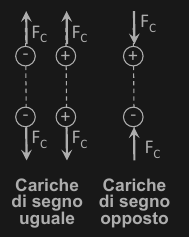
\includegraphics[scale=0.5]{Forza di Coulomb.png}
\end{center}

La forza di Coulomb $F_C$ è diretta nella direzione di $r$. Quando $q_1$ e $q_2$ hanno lo
stesso segno la forza di Coulomb è repulsiva. Quando sono di segno opposto la
forza è attrattiva.\\
L'unità di misura, nel Sistema Internazionale (SI), della forza di Coulomb è il
newton [N] ed il coefficiente di proporzionalità è $1/(4\pi \epsilon_0)$ dove $\epsilon_0$ è la costante dielettrica del vuoto [$\epsilon_0 = 8,854x10^{-12} C^2/(Nm^2)$].
\vspace*{0.2cm}\\
L'unità di misura della carica elettrica nel sistema di misura SI è il \textbf{coulomb} [C]. La carica elementare nel SI è $e$ ove
\[
    e = 1,6021 x 10^{-19} C
\]
Protone ed elettrone hanno carica di valore assoluto e. Due protoni o
due elettroni si respingono. Un protone ed un elettrone si attraggono.
Per convenzione la carica del protone è positiva ($+e$) e quella dell'elettrone negativa (-$e$).\\
In natura esistano solamente cariche multiple di e. Non può esistere
una carica sottomultiplo di $e$.



\subsubsection{La cariche elettriche ed il loro moto}
Forza che agisce su una particella carica:
\[
    \vec F = q(\vec E + \vec u \times \vec B)
\]
\begin{align*}
    &\vec F: \text{forza [N]} &
    &\vec q: \text{carica elettrica [C]} &
    &\vec u: \text{velocità della carica [m/s]}
\end{align*}
\begin{align*}
    &\vec E: \text{campo elettrico} &
    &\vec B: \text{vettore induzione magnetica}
\end{align*}
\begin{itemize}
    \item Se $\vec B=0$ si ha la cosiddetta \textbf{Forza elettrostatica}
    \[
        \vec F = q \vec E
    \]
    Quindi il campo elettrico $\vec E = \frac{\vec F}{q} $ è una forza per unità di carica [N/C].
    \vspace*{0.1cm}\\
    Campo elettrico e forza elettrostatica da cui esso deriva hanno la stessa
    direzione. Perciò il campo produce un'accelerazione della carica lungo la
    propria direzione.
    \vspace*{0.1cm}\\
    Nel SI l'unità di misura di $\vec E$ è: $N/C = V/ m = m \ kg \ s^{-2} C^{-1}$.
    \vspace*{0.2cm}\\
    \item Se $\vec E=0$ si ha la \textbf{Forza di Lorentz}
    \[
        \vec F = q(\vec u \times \vec B)
    \]
    Quindi il vettore induzione magnetica $\vec B$ è una forza per unità di carica e di velocità [$N s / C m$].
    Campo elettrico e forza elettrostatica da cui esso deriva hanno la stessa
    direzione. Perciò il campo produce un'accelerazione della carica lungo la
    propria direzione.
    Nel SI l'unità di misura di $\vec E$ è: $N/C = V/ m = m \cdot kg \cdot s^{-2} \cdot C^{-1}$.
\end{itemize}
Una particella carica induce una forza sulle cariche
che la circondano. Tale forza può essere attrattiva o
repulsiva. Essa è la forza Coulombiana $F_C$ (o forza
elettrostatica). In ogni punto della regione attorno
alla carica o in presenza ad una distribuzione di
cariche vi è un campo elettrico $\vec E(x,y,z)$ definito dalla
forza indotta su una carica di prova puntiforme
unitaria posta nel punto considerato.
\begin{center}
    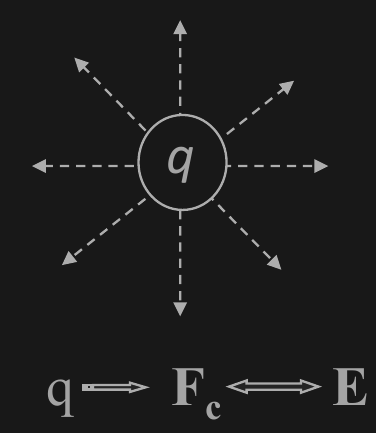
\includegraphics[scale=0.27]{Forza elettrostatica.png}
\end{center}
Qualora su una carica in moto si induca una forza
deviante perpendicolare al moto, tale forza è la
forza magnetica o forza di Lorentz 
$F_L$. Il campo
di induzione magnetica $\vec B(x,y,z)$, legato a $\vec F_L$, è
dato dalla forza indotta su una carica unitaria in
moto per unità di velocità della carica stessa. La
direzione del campo $\vec B$ è perpendicolare alla
velocità ed alla forza $\vec FL$ . Il campo $\vec B$ è
perpendicolare alla velocità della carica ed alla
forza indotta.

\subsection{Densità volumetrica di carica}
La carica elettrica non può essere creata o distrutta (legge della
conservazione della carica elettrica). Può solo essere trasferita. Pertanto, la
carica elettrica totale di un sistema isolato non può variare.\\
La densità volumetrica di carica (o distribuzione di carica) è definita da:
\[
    \rho_C (x,y,z) = \lim_{\Delta t \rightarrow 0} \frac{\Delta q}{\Delta \tau} = \frac{dt}{dq}  
\]
dove $d \tau$ è l'elemento infinitesimo di volume.

\subsubsection{Densità di corrente \texorpdfstring{$J$}{J}}
La densità di corrente elettrica $\vec J$ è il vettore il cui modulo è la quantità di
carica che attraversa una superficie unitaria perpendicolare alla velocità $\vec u$
delle cariche. La direzione ed il verso di $\vec J$ sono la direzione ed il verso di $\vec u$:
\[
    \vec J \cdot \hat n = \lim_{\Delta S \rightarrow 0} \lim_{\Delta t \rightarrow 0} \frac{\Delta Q}{\Delta S \Delta t}
\]
$\vec J$: densità di corrente $\left[\frac{C}{m^2\cdot s}\right] = \left[\frac{A}{m^2} \right]$

\begin{center}
    \includegraphics[scale=0.5]{Densità di corrente.png}
\end{center}

$\vec J(x,y,z)$ definisce un campo vettoriale ed è la densità di flusso delle
cariche. La corrente elettrica $i$ è il flusso di carica attraverso una
superficie $S$:
\[
    i = \iint\limits_S \vec J \cdot \hat n \ dS
\]




\subsection{Corrente elettrica}
La corrente elettrica i che attraversa una superficie è la quantità di carica
che attraversa la superficie nell’unità di tempo:
\[
     i = \frac{\Delta q}{\Delta t} 
\]
Se si considera un cavo conduttore, ad esempio, la corrente nel conduttore è la
quantità di carica che attraversa una sezione del cavo nell'unità di tempo.

\begin{center}
    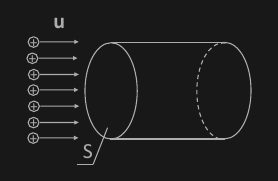
\includegraphics[scale=0.5]{Corrente conduttore.png}
\end{center}

L'unità di misura SI è l'ampere [$A$] dove $A = \frac{C}{s}$
\vspace*{0.1cm}\\
La \textbf{corrente elettrica istantanea} è:
\[
    i(t) = \lim_{\Delta t \rightarrow 0} \frac{\Delta q}{\Delta t} = \frac{dq}{dt}
\]



\subsection{Tensione elettrica e differenza di potenziale elettrico}
La \textit{tensione elettrica} $e_{12}$ fra i punti 1 e 2 lungo il
percorso $l$, è il lavoro $L^{1\rightarrow 2,l}_{q=1}$ che il campo elettrico
$\vec E(x,y,z)$ compie per portare una carica unitaria dl
punto 1 al punto 2 lungo $l$:
\[
    e_{12} = \int_{1,l}^2 \vec E \cdot d \vec l
\]

\begin{center}
    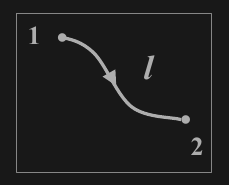
\includegraphics[scale=0.5]{Tensione.png}
\end{center}

Per spostare la carica $q$ dal punto 1 al 2 il lavoro è:
\[
    L^{1 \rightarrow 2,l}_q = q \cdot e_{12}
\]
L'unità di misura SI di $e_{12}$ è il volt [$V$] dove $V = \frac{J}{C} = m^2 \cdot kg \cdot s^{-2} \cdot C^{-1}$.
Qualora la tensione e 12 dipenda dai valori di una
funzione $v(x,y,z)$ definita in una regione che contiene la linea $l$ essa diviene:
\[
    e_{12} = \int_{1,l}^{2}\vec E \ d\vec l = - \int_{1,l}^{2} dv = v_1 - v_2 = v_{12}
\]
dove $v(x,y,z)$ è la \textbf{funzione potenziale elettrico} e $v_{12}$
è la \textbf{differenza di potenziale elettrico}.
\vspace*{0.1cm}\\
Poiché $v_{12}$ è la differenza fra i valori che la funzione $v(x,y,z)$ assume nel punto
iniziale e nel punto finale di $l$, $v_{12}$ non dipende dal percorso che unisce i due
punti. Quindi il campo $\vec E$ è un \textbf{vettore conservativo} \footnote{un campo conservativo è un campo il cui integrale lineare è indipendente dalla traiettoria} con $\vec E = \vec \nabla \cdot v(x,y,z)$.
\vspace*{0.1cm}\\
Per un percorso chiuso $l_c$ contenuto nella regione ove $\vec E$ è conservativo, si ha:
\[
    e_l = \oint _{l_c} \vec E \cdot d \vec l_c = - \oint _{l_c} \vec \nabla \cdot v  \ d\vec l_c = 0
\]



\subsection{Legge di Ampere-Prima legge di Maxwell}
La grandezza vettoriale campo magnetico H è definito dalla legge di Ampere (prima legge di Maxwell)
\[
    \oint _{l_c} \vec H \ d \vec l_c = i_t
\]
dove la corrente totale $i_t = i + i_s$.\\
In questo caso la corrente totale $i_t$ è il flusso del vettore $J_t$ i ovunque solenoidale ($J_t = J + \partial D/ \partial t$). Perciò $i_t$ è il flusso concatenato con la linea chiusa $l_C$ contorno della superficie che attraversa. Il verso di percorrenza di $l$ è determinato con regola della vite destrogira.
\begin{center}
    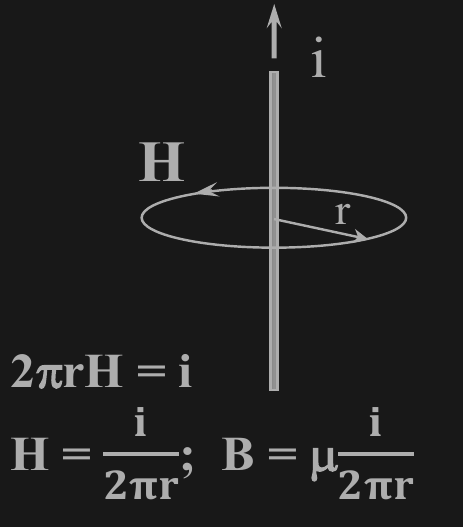
\includegraphics[scale=0.3]{Campo magnetico.png}
    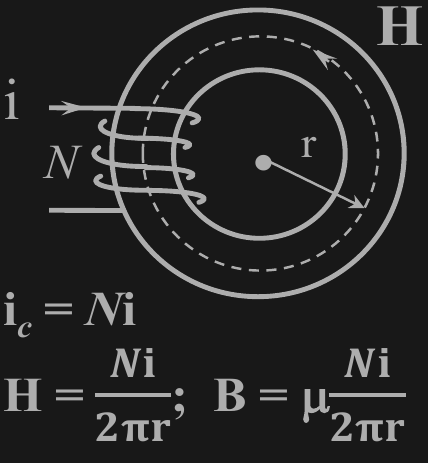
\includegraphics[scale=0.3]{Campo magnetico-2.png}
\end{center}
L'unità di misura SI di $\vec H$ è l'ampere su metro [$\frac{A}{m}$].
Per materiali lineari: $\vec B = \mu \vec H$ ove $mu$ è la permeabilità magnetica del materiale. Per mezzi non lineari
$\vec B = f(\vec H)$. Solitamente per i materiali magnetici non lineari $f$ è una funzione \textbf{isteretica} (materiali
ferromagnetici).
\begin{align*}
    \oint_{l_C}\vec H \ d \vec l &= \iint\limits_{S} \left( \vec J + \frac{\partial
    D}{\partial t} \right) \ \hat n \ dS\\
    &= \underbrace{\iint\limits_{S} \vec J \ \hat n \ dS}_{\text{corrente di conduzione } I} + \underbrace{\iint\limits_{S} \frac{\partial D}{\partial t} \ \hat n \ dS}_{\iint\limits_{S} \partial D \ \hat n \ dS =\vec \Phi(D)} =\\
    &= I + \underbrace{\frac{\partial \vec \Phi(D)}{\partial t}}_{\text{corrente di spostamento}}
\end{align*}
Immaginiamo di descrivere due superfici $S_1$ e $S_2$ sulla linea chiusa $l_C$
\[
    \oint_{l_C} \vec H \ d\vec l = \iint\limits_{S_1}\left( \vec J + \frac{\partial D}{\partial t} \right) \hat n_1 \ dS_1 = \iint\limits_{S_2}\left( \vec J + \frac{\partial D}{\partial t} \right) \hat n_2 \ dS_2
\]
Prendiamo una superficie chiusa $S_C$ su $S_2$, allora
\[
    \oint_{S_C}\underbrace{\bigg( \vec J + \frac{\partial D}{\partial t}\bigg)}_{\text{vettore solenoidale}}\hat n_C \ dS_C = \iint\limits_{S_2}\left( \vec J + \frac{\partial D}{\partial t} \right) \hat n_2 \ dS_2 - \iint\limits_{S_1}\left( \vec J + \frac{\partial D}{\partial t} \right) \hat n_1 \ dS_1 = 0
\]



\subsection{Legge dell'induzione di Faraday-Seconda legge di Maxwell}
La legge dell'induzione (o legge di Faraday
od anche seconda legge di Maxwell)
stabilisce che:
\[
    e_{l_C} = \oint_{l_C}
    \vec E \ d\vec l_C = -\frac{d \Phi}{dt}
\]
\begin{center}
    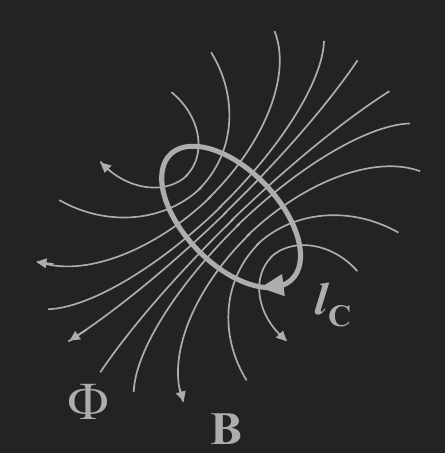
\includegraphics[scale=0.5]{Legge di Faraday.png}
\end{center}
ove $\Phi$ è il flusso magnetico concatenato con
la linea chiusa $l_c$. (direzione di $l_C$ data dalla
regola della vite destrogira).\\
$e_{l_c}$ è la tensione elettrica indotta sulla
linea chiusa dalla variazione del flusso
magnetico concatenato con $l_c$; essa è detta
\textbf{forza elettromotrice} (f.e.m.).
\vspace*{0.1cm}\\
\textbf{N.B.} In questo caso $\vec E$ non à conservativo.



\subsection{Conservazione della carica elettrica}
La carica elettrica non si crea né si distrugge. Perciò la diminuzione della carica elettrica
all'interno di un volume $\tau$ corrisponde alle
cariche che lasciano $\tau$ fluendo attraverso la
superficie chiusa $S$, superficie esterna di $\tau$.
\begin{center}
    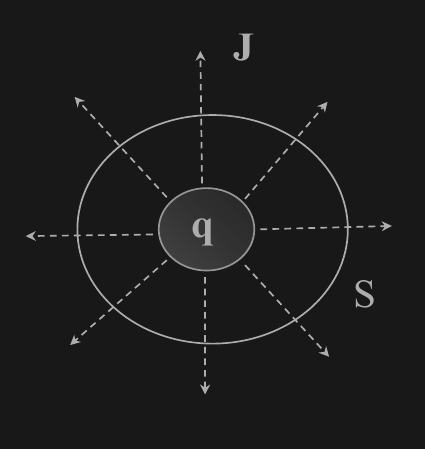
\includegraphics[scale=0.5]{Conservazione della carica.png}
\end{center}
La \textbf{\textit{
legge di conservazione della carica elettrica}} afferma questo ed è espressa
dall'espressione: 
\[
    \oiint_{S} \vec J \ \hat n \ dS = - \frac{dQ}{dt}
\]
si ha variazione di cariche solo se c'è passaggio di corrente.




\subsection{Legge di Gauss}
Il campo di induzione elettrica o campo spostamento elettrico è definito dalla
legge di Gauss.
Considerando una superficie chiusa $S$,
che delimita il volume $V$; sia $\hat n$ il versore
normale alla superficie. La legge di Gauss
afferma che:
\[
    \oiint_{S} \vec D \ \hat n \ dS = \iiint_{V}\rho \ dV = Q
\]



\subsection{Forza elettromotrice}
$\vec E$ e $\vec B$ descrivono le forze prodotte dal fenomeno elettromagnetico sulle
cariche (forza elettrica per unità di carica e forza magnetica per unità di
carica e di velocità della carica). Esse descrivono ciò che viene prodotto dal
fenomeno EM. Ne descrivono l'\textbf{effetto}.
\vspace*{0.1cm}\\
$\vec D$ ed $\vec H$ descrivono ciò che produce il fenomeno EM (la carica elettrica nel
primo caso e la corrente totale nel secondo). Ne descrivono la \textbf{causa}.

\subsection{Leggi dell'Elettromagnetismo in forma integrale}
\renewcommand{\arraystretch}{2.5}
\begin{center}
    \begin{tabular}{|c|c|}
        \hline
        $\oint_{l_c} \vec H \ d \vec l_c = i_t$ & $1^o$ legge di Maxwell\\
        \hline 
        $\oint_{l_c} \vec E \ d \vec l_c = \dfrac{d\Phi}{dt}$ & $2^o$ legge di Maxwell\\
        \hline
        $\oiint \vec J \ \hat n dS = - \dfrac{dq}{dt}$ & legge di conservazione della carica \\
        \hline
        $\oiint \vec D \ \hat n dS = q $ & legge di Gauss\\
        \hline 
        $\oiint \vec J_t \ \hat n dS = 0 $ & $\vec Jt$ ovunque solenoidale\\
        \hline t
        $\oiint _S \vec B \ \hat n dS=0$ & $\vec B$ ovunque solenoidale\\
        \hline
    \end{tabular}    
\end{center}
Tre di queste sei equazioni sono linearmente indipendenti, le altre tre si ottengono dalle prime tre.



\subsection{Leggi dell'Elettromagnetismo in forma locale}
\begin{center}
    \begin{tabular}{|c|c|}
        \hline
        $\nabla \times \vec H = \vec J + \dfrac{\partial
        \vec D}{\partial t}$ & 1° legge di Maxwell (dal teorema di Stokes) \\
        \hline 
        $\nabla \times \vec E = - \dfrac{\partial
        \vec B}{\partial t}$ & 2° legge di Maxwell
        (dal teorema di Stokes)\\
        \hline
        $\nabla \cdot \vec J = - \dfrac{\partial \rho_c}{\partial t} $ & legge di conservazione della carica (teor. divergenza)\\
        \hline
        $\nabla \cdot \vec D = \rho_c$ & legge di Gauss (dal teorema della divergenza)\\
        \hline
        $\nabla \cdot \vec J_t = 0$ & $\vec J_t$ ovunque solenoidale (dal teorema della divergenza)\\
        \hline 
        $\nabla \cdot \vec B =0$ & $\vec B$ ovunque solenoidale (dal teorema della divergenza)\\
        \hline
    \end{tabular}    
\end{center}
Tre di queste sei equazioni sono linearmente indipendenti, le altre tre si ottengono dalle prime tre.



\subsection{Relazioni materiale}
$\vec E$ e D, $\vec B$  ed $\vec H$  descrivono i fenomeni dell'EM in modo diverso. $\vec E$ e $\vec D$ si
riferiscono al fenomeno Elettrico, $\vec B$  ed $\vec H$  al fenomeno magnetico. $\vec D$ ed $\vec H$ 
descrivono i due fenomeni misurando ciò che li origina: la carica il primo, ed il
moto della carica il secondo. Gli effetti misurati da $\vec E$ e da $\vec B$  sono in entrambe i
casi le forze indotte. Essi dipendono da come i diversi materiali reagiscono.
Inoltre, dipendentemente dalla proprietà del materiale, ad un certo valore del
campo $\vec E$ si induce un determinato moto di carica misurato da $\vec J$ . Le relazioni
fra queste descrizioni spesso sono lineari. A volte però non lo sono con
relazioni anche di tipo Isteretico.
\begin{center}
    \begin{tabular}{|c|c|}
    \hline
    \textbf{Materiali lineari} & \textbf{Materiali non lineari}\\
    \hline 
    $\vec D = \epsilon \vec E$ & $\vec D = f_1(\vec E)$\\
    \hline 
    $\vec B = \mu \vec H$ & $\vec B = f_2(\vec H)$\\
    \hline 
    $\vec J = \sigma \vec E$ & $\vec J = f_3(\vec E)$\\
    \hline
\end{tabular}
\end{center}
con $\epsilon$ costante dielettrica, $\mu$ permeabilità magnetica e $\sigma$ conducibilità termica.
\vspace*{0.1cm}\\
la costante dielettrica (permittività elettrica) $\epsilon$, e la permeabilità magnetica $\mu$
di un materiale sono espresse per mezzo dei loro valori relativi $\epsilon_r$ ed $\mu_r$ in riferimento al loro valore nel vuoto $\epsilon_0$ ed $\mu_0$:
\begin{align*}
    &\epsilon = \epsilon_r \epsilon_0 &\text{dove } \epsilon_0 = 8,856 x 10^{-12} Farad/metro \left[\frac{F}{m}\right]\\
    &\mu = \mu_r \mu_0 &\text{dove } \mu_0 = 1,256 x 10^{-6} Henry/metro \left[\frac{H}{m}\right]
\end{align*}
Riporto alcuni valori di $\epsilon_r$
\begin{center}
    \renewcommand{\arraystretch}{1}
    \begin{tabular}{c|c}
         & $\epsilon_r$\\
        \hline
        vuoto & 1\\
        aria & $\simeq 1$\\
        plastica & 2-5\\
        vetro & 4-8\\
        acqua & 80
    \end{tabular}
\end{center}
Molto diverse sono le variazioni per materiali differenti della
conducibilità elettrica, della permeabilità magnetica e della costante
dielettrica.
Per la conducibilità elettrica $\sigma$ vi è una variazione anche di $10^{23}$ (23 ordini
di grandezza) fra materiali isolanti e materiali conduttori.
Per la permeabilità magnetica $\mu$ la variazione raggiunge al massimo un
valore di circa $10^5$ (5 ordini di grandezza).
Per la costante dielettrica $\epsilon$ la variazione massima si riduce ad un valore
massimo di circa $10^3$ (3 ordini di grandezza).
\vspace*{0.2cm}\\
La relazione fra $\vec J$ ed $\vec E$ è
anche definita dalla
resistività elettrica $\rho$:
\[
    \vec E = \rho \vec J
\]
dove
$\rho = \frac{1}{\sigma}$
$\sigma$ è in Siemens/metro [$\frac{S}{M}$] e $\rho$ in Ohm/metro [$\frac{\Omega}{m}$].


\subsection{SI Units}
\subsubsection{Unità derivate SI}

    \begin{tabular}{|m{35mm}|c|c|m{35mm}|}
    \hline
    Grandezza&
    Simbolo (nome)&
    Unità SI non di base&
    Unità SI di base\\
    \hline 
    Carica elettrica&
    $C$ (Coulomb)&
    & 
    $s \times A$\\
    \hline
    Tensione elettrica e differenza di potenziale elettrico&
    $V$ (Volt)&
    $ \dfrac{W}{A}$&
    $m^2 \times kg \times s^{-3} \times A^{-1}$\\
    \hline
    Forza&
 $N$ (Newton)&
 &
 $m \times kg \times s^{-2}$\\
 \hline
Energia/Lavoro&
 $J$ (Joule)&
 $N \times m$&
 $m^2 \times kg \times s^{-2}$\\
 \hline
Potenza&
 $W$ (Watt)&
 $\dfrac{J}{s}$&
 $m^2 \times kg \times s^{-3}$\\
 \hline 
Flusso magnetico&
 $Wb$ (Weber)&
 $V \times s$&
 $m2 \times kg \times s-2 \times A^{-1}$\\
 \hline 
Induzione magnetica&
 $T$ (Tesla)&
 $\dfrac{Wb}{m^2}$&
 $kg \times s^{-2} \times A^{-1}$\\
 \hline 
Resistenza elettrica&
 $\Omega$ (Ohm)&
 $\dfrac{V}{A}$&
 $m^2 \times kg \times s^{-3} \times A^{-2}$\\
 \hline 
Conduttanza elettrica&
 $S$ (Siemens)&
 $\dfrac{A}{V}$&
 $m^{-2} \times kg^{-1} \times s^3 \times A^2$\\
 \hline 
Capacità&
 $F$ (Farad)&
 $\dfrac{C}{V}$&
 $m^{-2} \times kg^{-1} \times s^4 \times A^2$\\
 \hline 
Induttanza&
 $H$ (Henry)&
 $\dfrac{Wb}{A}$&
 $m^2 \times kg \times s^{-2} \times A^{-2}$\\
 \hline
Frequenza&
 $Hz$ (Hertz)&
 &
 $s^{-1}$\\
 \hline 
\end{tabular}


\subsubsection{Prefissi SI}
\begin{center}
    \renewcommand{\arraystretch}{1.5}
    \begin{tabular}{|c|c|c|}
        \hline
        Factor & Name & Symbol\\
        \hline 
        $10^{-24}$ & yocto  & y\\
        \hline 
        $10^{-21}$ & zepto & z\\
        \hline 
        $10^{-18}$ & atto & a\\
        \hline 
        $10^{-15}$ & femto & f\\
        \hline 
        $10^{-12}$ & pico & p\\
        \hline 
        $10^{-9}$ & nano & n\\
        \hline 
        $10^{-6}$ & micro & $\mu$\\
        \hline 
        $10^{-3}$ & milli & m\\
        \hline 
        $10^{-2}$ & centi & c\\
        \hline 
        $10^{-1}$ & deci & d\\
        \hline 
        $10^{1}$ & deca & da\\
        \hline 
        $10^{2}$ & hecto & mh\\
        \hline 
        $10^{6}$ & mega & M\\
        \hline 
        $10^{9}$ & giga & G\\
        \hline 
        $10^{12}$ & tera & T\\
        \hline 
        $10^{15}$ & peta & P\\
        \hline 
        $10^{18}$ & exa & E\\
        \hline 
        $10^{21}$ & zetta & Z\\
        \hline 
        $10^{24}$ & yotta & Y\\
        \hline 
    \end{tabular}
\end{center}
prova



































\end{document}